\chapter{Spatial Early Warning Signals}
\graphicspath{{spatial_ews/figs}}

\section{Fast and Slow Tipping Elements}
An open question in the theory of Early Warning Signals is how to make use of them when the control parameter
changes quickly relative to the timescale of the system\cite{VanderBolt2021}\todo{I should read this paper properly}.
To be more formal about this, consider the system
\begin{equation}
  \label{eq:system_with_a_timescale}
  \dv{y}{t} = \frac{f(y,rt)}{T}
\end{equation}
where $y$ is the system state, $T$ is a characteristic timescale of the system and $r$ is the rate the system is linearly forced
at. Suppose further than there is a tipping point at time $t = t^*$ (i.e.\ when the forcing reaches a magnitude of $rt^*$). By considering
the ratio of the system to forcing timscale we can define a parameter $\epsilon = rT$ and introduce a rescaling of time $t=Ts$
so that \cref{eq:system_with_a_timescale} becomes
\begin{equation}
  \label{eq:system_with_a_timescale_rescaled}
  \dv{y}{s} = f(y,\epsilon s).
\end{equation}

There is an important limit to be considered here. Suppose $r$ is very small --- in other words the system is forced very slowly --- so that we
can take $\epsilon\rightarrow 0$ in such a way that $\epsilon s \rightarrow \mu$ where $\mu$ is a constant. We can now view this as a bifurcation
problem and can then apply all the usual tools to detect approaching tipping points\cite{scheffer2009}.

This limit of slow forcing can also be viewed as the limit of a system with a very rapid timescale. Hence tipping point assossiated to the system
this limit applies to (whether because it is slowly forced or rapidly responding) is known as a \emph{fast tipping point}.

Alternatively we can look at so called \emph{slow tipping elements} in which $\epsilon$ is not small. It is difficult to get good Early Warning Signals
using the temporal variance and autocorrelation\cite{VanderBolt2021}. Unfortunately these sorts of systems are widespread in climate change science.
Recall that the rate of global warming is fast, on the order of \SI{1}{\kelvin} per century\cite{Osborn2021}, a rate unprecidented in
a long time\todo{find a good citation for this}. Many important tipping elements have timescales of centuries or longer\todo{cite timescales}.
This implies that for contemporary climate change $\epsilon$ is unlikely to be small. This motivates the development of technqiues that enable
larger values of $\epsilon$ to be probed.

Part of the problem with these slow tipping elements is that the forcing changes appreciably over the window used to calculate early warning signals.
To get around this we might try to make `instantaneous' measurements of its variance and autocorrelation. One way to do this would be to calculate these
statistics over space instead of over time.

\section{Prior Work}
\todo{What is known about spatial EWS already?}

\section{The System}
In order to investigate spatial early warning signals we will investigate a specific system. We will choose this system
to be generic enough that broader conclusions can be drawn. We will make the system as simple as possible to make it more
likely to give understandable results.

Making the hypothesis that near a tipping point many systems are governed by coherent dynamics leads us to introduce one dependent
variable $y$. In one dimension there is only one generic type of bifurcation\cite{Thompson1994}, the saddle node. Furthermore
near a saddle node bifurcation, all systems show qualitatively similar behaviour\cite{guckenheimer2013} so the dynamics of $y$ should
involve the lowest order terms which give a saddle node, namely $\dot{y} = y - y^3/3 - \mu$, where $\mu$ is a control parameter.

We need to take into account the spatial nature of the problem. Again to keep things simple, we will restrict attention to a 1 dimensional
periodic domain. To couple in space we use the well studied diffusive coupling which acts to smooth out the value of $y$.\todo{This can be
  better justified. Furthermore, something like: such a form has found numerous uses
in simple models for ecological and earth system applications: energy bal-
ance models for global temperature, models of the movement of species and
pattern formation in ecosystems.}

We will introduce noise into the system and assume the control parameter changes linearly with time. All of these considerations motivates studying
\begin{subequations}
\label{eq:spatial_system}
  \begin{align}
    \pdv{y}{t} &= y - \frac{1}{3}y^3 - \mu + D\pdv[2]{y}{x} + \sigma\zeta \label{eq:spatial_system_y} \\
    \dv{\mu}{t}&= \epsilon \label{eq:spatial_system_mu}
  \end{align}
\end{subequations}
where $\zeta$ is a white noise with mean $\langle \zeta(x,t) \rangle = 0$ and covariance $\langle \zeta(x,t)\zeta(x',t')\rangle = \delta(x-x')\delta(t-t')$\todo{check this}.
It therefore follows that $\sigma$ is the magnitude of the noise.

We set the size of the domain to be $L$. The variable $\mu$ linearly increases between $\mu = 0$ and $\mu = 1$ and so the system will undergo a saddle node
bifurcation at $\mu = 2/3$.

Alternatively, we can view the system variationally\footnote{A brief review of the concepts of the variational derivative are presented in \cref{appendix:variational_calculus}.}.
To do this we introduce the `energy'
\begin{equation}
  \label{eq:spatial_system_energy}
  \mathscr{E} = \int_0^L -\frac{1}{2}y^2 + \frac{1}{12}y^4 + \mu y + \frac{1}{2}D\left(\pdv{y}{x}\right)^2\,\mathrm{d}{x}.
\end{equation}

With this we can rewrite \cref{eq:spatial_system_y} as
\begin{equation}
  \label{eq:spatial_system_y_variational}
    \pdv{y}{t} = -\fdv{\mathscr{E}}{y(x)}  + \sigma\zeta, 
\end{equation}
which is a Time Dependent Ginzburg Landau equation\todo{cite this --- phase transitions book?}.

\section{Statistics}
We will compare the autocorrelation and variance of \cref{eq:spatial_system} calculated over space and over time. We will now
make precise what that means. For a summary see \cref{tab:ews_space_time_definition}.

\subsection{Spatial Statistics}

We will definte the average of a quantity calculated from \cref{eq:spatial_system}, $A(t) = A(y(x,t),x)$ in the obvious way
\begin{equation}
  \label{eq:definition_of_average}
  \langle A \rangle = \frac{1}{L}\int_0^L A(y(x,t),x) \,\mathrm{d}x.
\end{equation}
We can now define the spatial variance of $y$ at time $t$ as
\begin{equation}
  \label{eq:spatial_variance}
  \sigma_s(t)^2 = \langle y^2 \rangle - \langle y \rangle.
\end{equation}
We will define the autocorrelation over space as
\begin{equation}
  \label{eq:spatial_autocorrelation}
  \alpha_s(t) = \frac{\langle y(t,x)y(t+\Delta t,x) - \langle y(t,x)^2 \rangle }{\sigma_s(t)^2}.
\end{equation}
The quantity $\Delta t$ is the lag of the autocorrelation. However \cref{eq:spatial_system} will ultimately be solved numerically and
in everything that follows we will set $\Delta t$ to the timestep, so that $\alpha_s$ is the lag-1 autocorrelation.

\subsection{Temporal Statistics}
When working over time, we will convert the spatiotemporal data to temporal data by first averaging in space to get $\left\langle y \right\rangle$.
To calculate the early warning indicators over time, we must define averaging in time. Consider the quantity $B(t)$. We will
define the temporal average as
\begin{equation}
  \label{eq:definition_of_temporal_average}
  \overline{B} = \frac{1}{T}\int_0^TB(t)\,\mathrm{d}t
\end{equation}
where the average is taken over some suitable window of length $T$.

When computing early warning indicators, we must first `detrend' the timeseries. We denote the detrended time series of $\langle y \rangle$ as $z$.
The the variance and autocorrelation, defined over a window of length $\tau_w$ are
\begin{equation}
  \label{eq:temporal_variance}
  \sigma_t^2 = \overline{z^2} - \overline{z}^2 
\end{equation}
and
\begin{equation}
  \label{eq:temporal_autocorrelation}
  \alpha_t = \frac{\overline{z(t)z(t+\Delta t)}}{\sigma_t^2}.
\end{equation}
\begin{table}[h]
  \centering
  \begin{tabular}[h]{llll}
    \toprule
    Quantity        & Domain & Symbol        & Definition \\
    \midrule
    Variance        & Space  & $\sigma_s^2$  & $\langle y^2 \rangle - \langle y \rangle$ \\
    \rule{0pt}{4ex}    
                    & Time   & $\sigma_t^2$  & $\overline{z^2} - \overline{z}^2$ \\
    \rule{0pt}{4ex}    
    Autocorrelation & Space  & $\alpha_s$    & $\frac{\left\langle y\left(t,x\right)y\left(t+\Delta t,x\right)\right\rangle - \left\langle y\left(t,x\right)^2 \right\rangle}{\sigma_s(t)^2}$ \\
    \rule{0pt}{4ex}    
                    & Time   & $\alpha_t$    &  $\frac{\overline{z(t)z(t+\Delta t)}}{\sigma_t^2}$ \\
    \bottomrule
  \end{tabular}
  \caption[Definition of spatial and temporal early warning signals]{The definition of the early warning indicators, over space and over time}
  \label{tab:ews_space_time_definition}
\end{table}

\section{Numerical Results}
\subsection{Numerical Method}
To solve \cref{eq:spatial_system}, we discretise the domain into $N = 100$ grid
points and 
calculate the diffusive term with finite differences. We denote the value of $y$ at the $k$th gridpoint by $y_k$. We integrate forward in time by 
using an implicit Euler method, where we solve the resulting nonlinear equation using 
MINPACK's HYBRD method accessed through SciPy\cite{Virtanen2020}. To avoid excessively long integrations when $\epsilon$ is small,
we set the timestep $\delta t = 0.001/\epsilon$ and integrate until $t=1/\epsilon$. We
calculate all early warning signals from $\epsilon t=0$ until $\epsilon t=2/3$, which is the 
time of the tipping point. When working over time, we choose our window size to 
contain 500 data points (i.e.\ half the time series),
so that the window length is $\tau_w = 1/(2\epsilon)$. We perform a quadratic detrend in these windows.
To stand a chance of getting good early warning
signals in time we require that $\epsilon < 1/\tau_w$, which is always satisfied.
Systems are initialised in equilibrium and spun up for 1000 time steps.
\subsection{Two Limits}
Before fully exploring the effect of $\epsilon$ and $D$ on early warning signals, we will look at two important limits.    
\subsubsection{Uncoupled Limit}
We will  begin by examining the case when $D = 0$, for large and small values of $\epsilon$. Consider \cref{fig:uncoupled_timeseries}.
\begin{figure}[h]
  \centering
  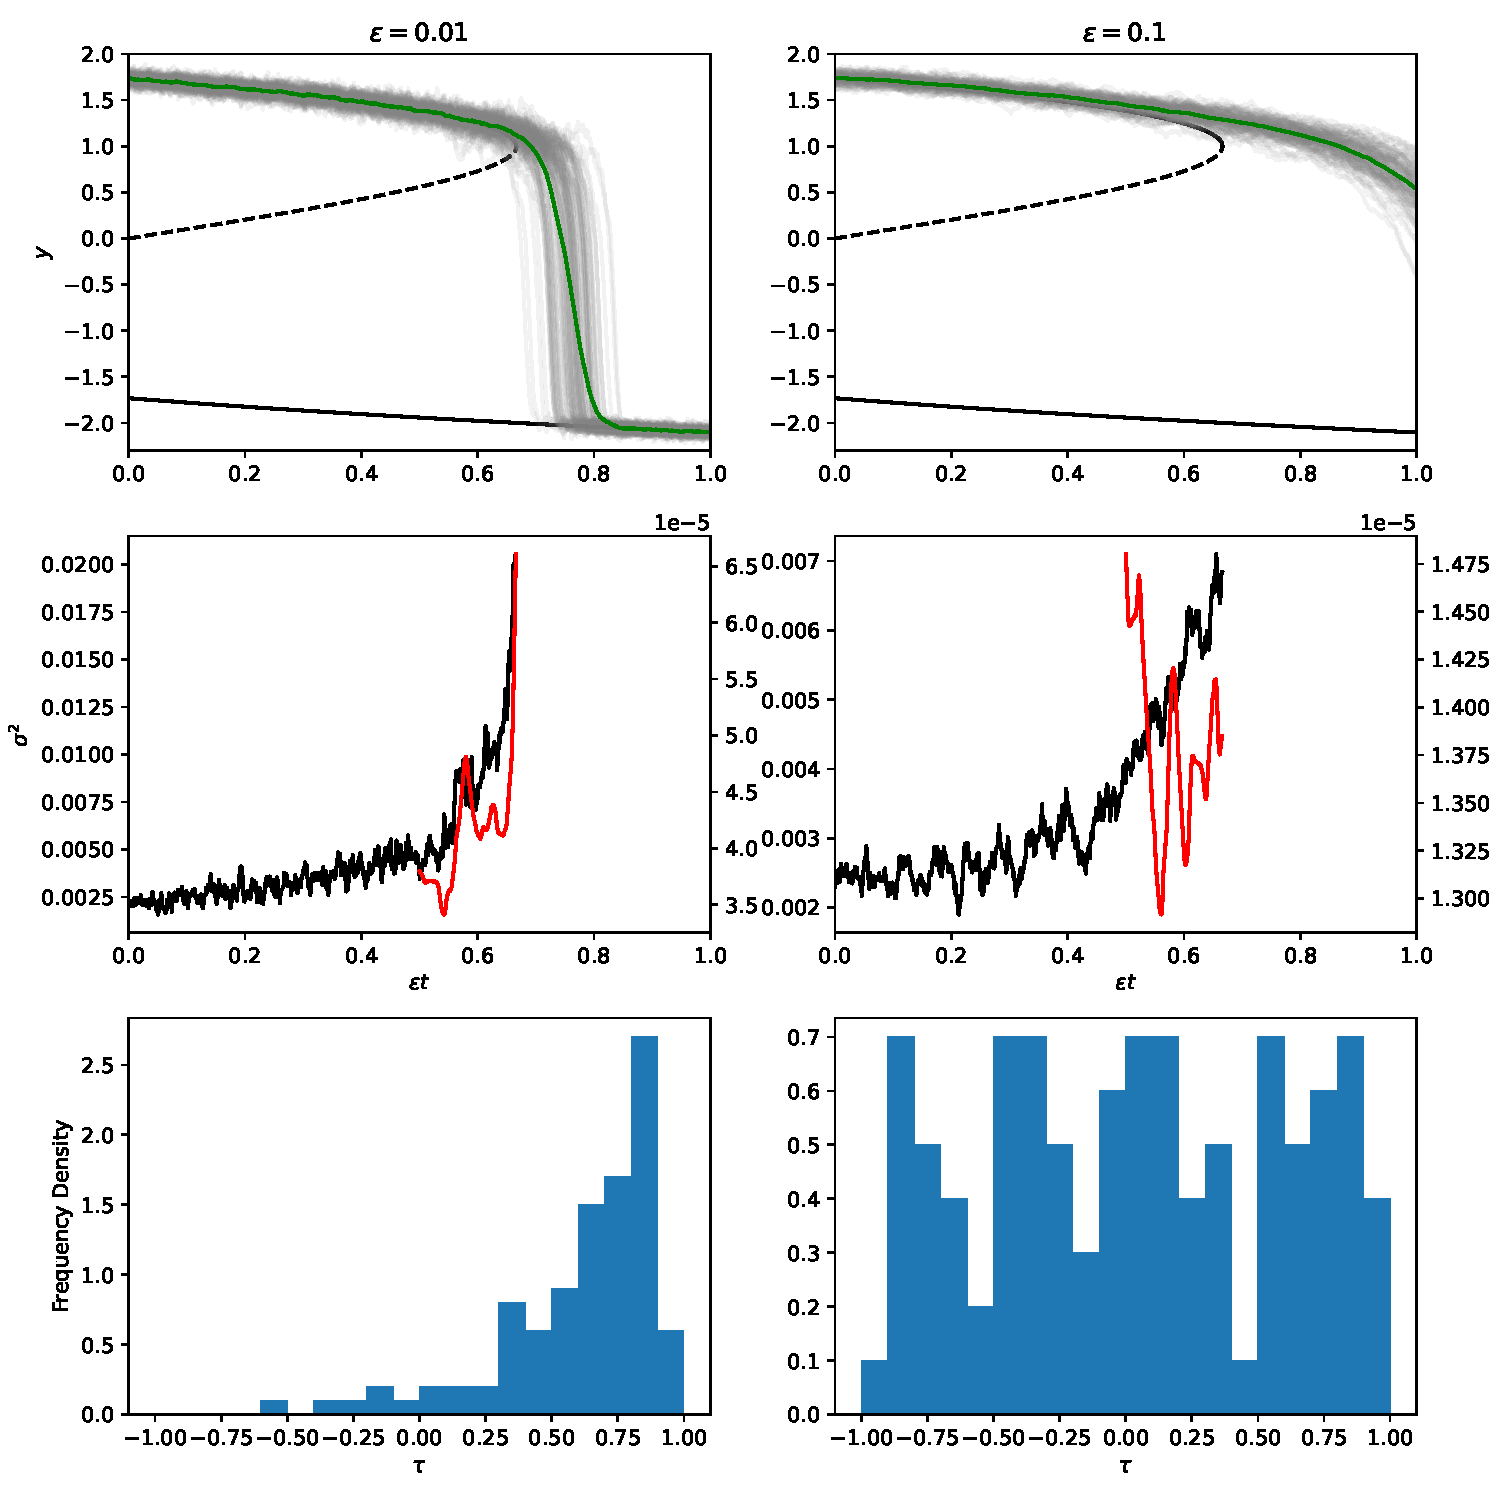
\includegraphics[width=\textwidth,keepaspectratio]{uncoupled_variance}
  \caption[Early warning signals in the uncoupled limit]{Early warning signals when $D = 0$. The left column shows the slow forcing case and the right column shows the fast forcing.
    The top row shows the individual trajectories with the mean trajectory shown in green. The black curves are the quasistatic equilibria.
    In the second row the we plot $\sigma_s^2$ in black and $\sigma_t^2$ in red. In the bottom row we calculate $\sigma_t^2$ from the individual
    $y_k$ values rather than the mean and calculate the kendall $\tau$ value for each and plot a histogram of the results. The mean $\tau$ values
                are 0.6 and 0.04 for the slow and fast case respectively.}
  \label{fig:uncoupled_timeseries}
\end{figure}
 The left column shows the small $\epsilon$ case. This is the case
    where we expect temporal early warning signals to work well. For this value of $\epsilon$ the system
    transitions to its new state near the time of the bifurcation and its variance calculated over
    space or calculated over time both clearly increase near the bifurcation point. Furthermore
    calculating the statistics for each the individual grid points shows that most grid points 
    experience a rise in variance over time as well.

    For the larger $\epsilon$ case the results are different. The system has not yet transitioned to
    its new state even by the end of the simulation. We do not see a clear rise in $\sigma_t^2$ near the bifurcation point. Furthermore looking at the individual grid points
    we do not see a coherent warning of the upcoming transition. However there is a very clear rise in $\sigma_s^2$ before the bifurcation, demonstrating that spatial early warning
    signals are superior in this case.

    \subsubsection{Slowly Forced Limit}
    \begin{figure}[h]
      \centering
      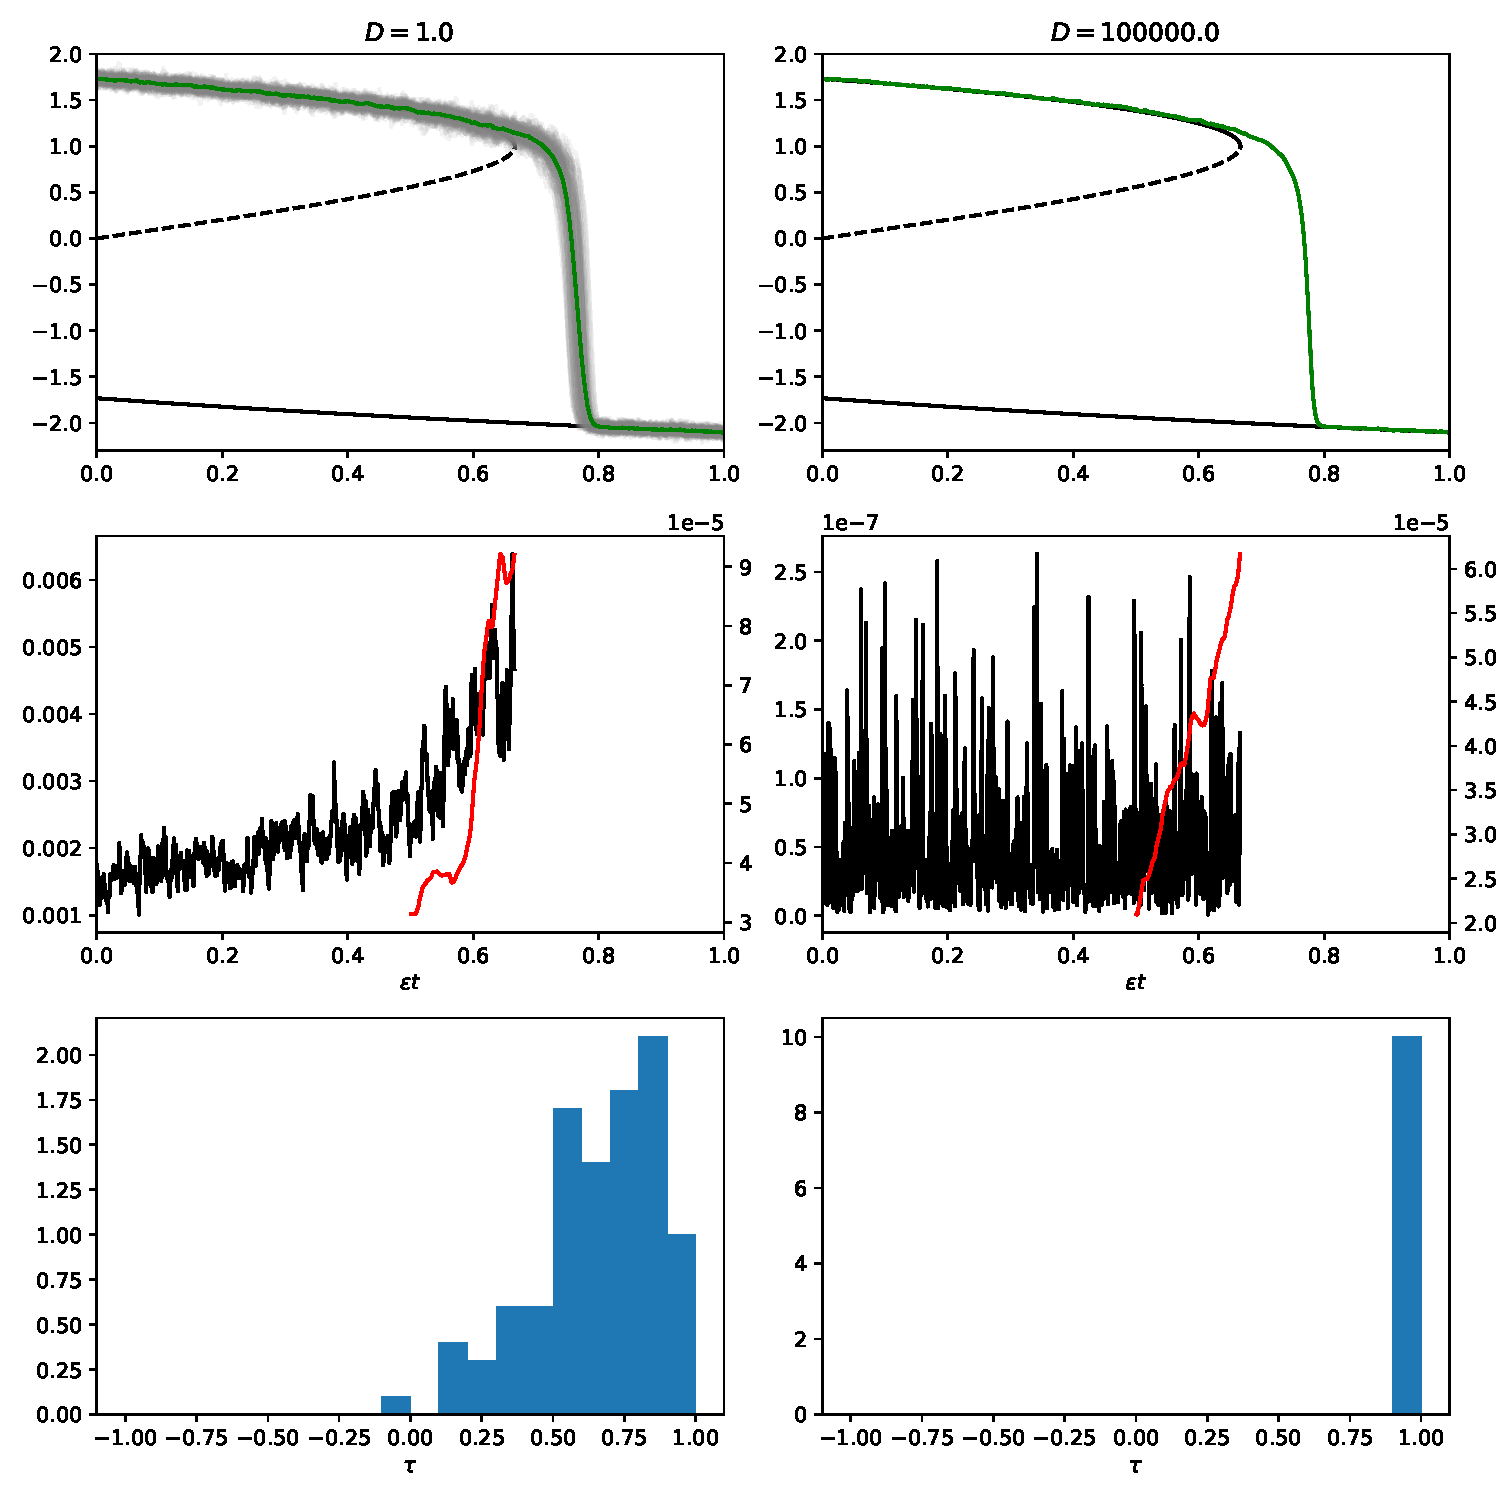
\includegraphics[width=\textwidth,keepaspectratio]{coupled_variance}
      \caption[Early Warning Signals in the slowly forced limit]{Early warning signals when $\epsilon = 0.01$. The left column shows 
                the weakly coupled case, the right shows what happens in the strongly coupled (large $D$) case. 
                The top row shows the quasi-static equilibria (black) the individual
                trajectories of the grid boxes (grey) and the domain average (green).
			      The variance is plotted in the second row, calculated over space 
                (black) and over time (red). The bottom row shows a histogram of the kendall $\tau$ values calculated over time for each $y_k$.}
              \label{fig:coupled_variance}
    \end{figure}
\subsection{Exploring the $\epsilon$ and $D$ parameter space}
\subsubsection{Scaling Arguments}
\section{Discussion}
\section{Conclusion}
